\section{Related Work}

\paragraph{Uncertainty estimation for LLMs.}
Output-based estimators score uncertainty from a single sequence
through token-level probability, predictive entropy, length-normalized
scoring, or SAR
\citep{malinin2021uncertainty,duan2024shifting,schweighofer2025rethinking},
or from semantic agreement across multiple samples
\citep{kuhn2023semantic,lin2024generating,jiang2024,nguyen2025snne};
recent work trims the 5--20-generation cost with diversity-promoting
or beam-based proposals
\citep{aichberger2025sdlg,park2025diversity,fadeeva2026beams} and
folds in cross-model disagreement to catch confident errors
\citep{hamidieh2026crossmodel}. Both families exhibit systematic length
bias even after normalization
\citep{vashurin2025line,santilli2025lengthbias} and decouple uncertainty
from the model's internal state, which motivates \emph{mechanistic}
estimators that read hidden representations directly. A first wave of
probes treats a single layer--token slice as input and separates truth
from error in the residual stream
\citep{kadavath2022,azaria2023,burns2022,marks2023,li2024,ji2024,liu2024,chen2024,orgad2024}.
Subsequent work widens this slice along several complementary axes:
ACT-ViT \citep{barshalom2025} pools the full layer--token plane as an
activation image through a Vision Transformer; fact-probe pushes
detection to claim-level granularity
\citep{snyder2024,he2024,han2025factprobe}; attention-based variants
exploit cross-token focus patterns
\citep{li2025uqac,duan2024shifting,yuksekgonul2023,sriramanan2024attention,vazhentsev2025rauq};
and feature-gap methods compare representations across contexts to
expose epistemic uncertainty
\citep{bakman2025featuregaps,gottesman2024,slobodkin2023,simhi2024}.
The common limitation is one score per response (or one forward per
claim, Figure~\ref{fig:inference_time}), which dilutes the signal as
responses grow long (Figure~\ref{fig:perf_by_length});
Figure~\ref{fig:signal_propagation} shows that the relevant activation
signal extends across tokens on both sides of a hallucinated span --
the structural fact that motivates our windowed formulation.

\paragraph{Uncertainty in long-form generation.}
Long responses interleave correct and uncertain content, which
single-score detectors cannot localize. Decomposition is the standard
remedy: at the claim level via atomic-fact extraction
\citep{min2023,wei2024,zhao2024} or conformal claim-level prediction
\citep{mohri2024}; at the sentence level by re-applying
self-consistency per sentence \citep{manakul2023,band2024}; and at
the token level via per-token probes \citep{he2024,su2024}. The
trade-off is real: claim and sentence pipelines depend on an external
extractor and one model call per unit, while token-level methods are
the only ones compatible with real-time generation -- though noisier
when read in isolation. We make the token level usable in practice by
sharing computation across a window of tokens rather than scoring each
in isolation, and by training under weakly supervised temporal
localization.

\paragraph{Weakly-supervised temporal localization.}
Our localization mechanism follows WTAL in video understanding, where
only video-level labels are available and per-frame relevance must be
inferred. \citet{pilhyeonlee2021} cast WTAL as uncertainty modelling,
treating background frames as out-of-distribution and aggregating
per-frame scores with multiple-instance learning. The analogy with
hallucination detection is direct: only response-level labels are
available, yet per-window uncertainty must be inferred. We treat
generated tokens as the temporal axis and aggregate per-window logits
with top-$k$ MIL.

\begin{figure}[t]
\centering
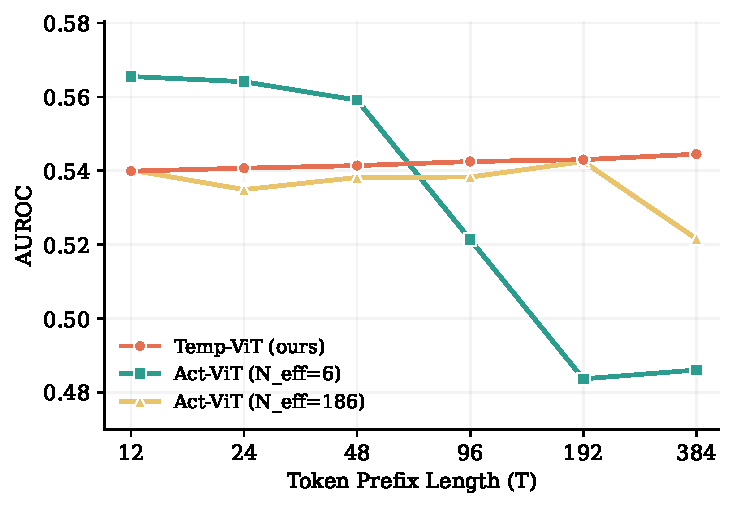
\includegraphics[width=0.95\linewidth]{figs/fig_perf_by_length.pdf}
\caption{Per-token AUROC on the LongFact prefix-truncation test as the
generated-token prefix length $T$ fed to each model grows. ACT-ViT
with its default short pooled token axis (\emph{Act-ViT, N\textsubscript{eff}=6})
peaks at short prefixes but collapses past $T = 48$ and falls below
chance for $T \in \{192, 384\}$ as the pooling compresses an
increasing number of token positions into the same fixed-size image.
Raising the pooled axis (\emph{Act-ViT, N\textsubscript{eff}=186})
partially rescues long prefixes but does not match Temp-ViT's flat
profile, which is per-token by construction. This illustrates the
long-form weakness of activation-tensor methods that pool the token
axis into a fixed-size representation.}
\label{fig:perf_by_length}
\end{figure}

\begin{figure}[t]
\centering
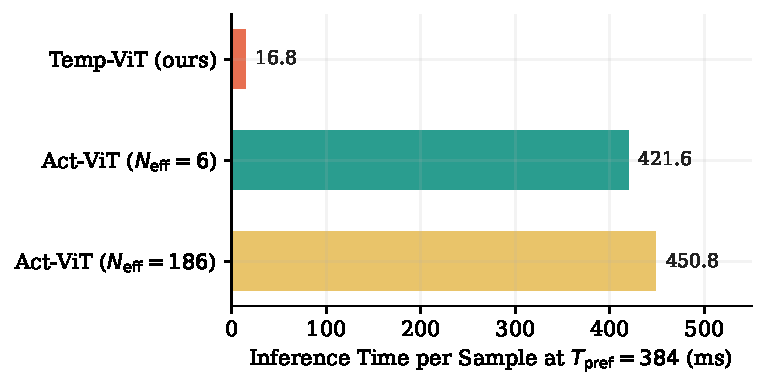
\includegraphics[width=0.95\linewidth]{figs/fig_inference_time.pdf}
\caption{Wall-clock time to score every token of one $T = 384$-token
LongFact passage on a single H200, batch~1, FP32. ACT-ViT emits one
scalar per call, so labelling every token requires $T$ sequential
forwards; per-call latency is small but the total scales linearly with
the response length, even when the post-pool ViT input is widened to
recover long-range accuracy (\emph{N\textsubscript{eff}=186}).
Temp-ViT produces the full per-token logit vector in a single forward
pass and is roughly $25\times$ faster on this passage, illustrating
the real-time-cost weakness of activation-tensor methods that need one
call per generated token.}
\label{fig:inference_time}
\end{figure}

